\section{Aufbau und Durchführung}
\subsection{Aufbau}
\label{sec:Aufbau}

Der Versuchsaufbau zum Millikan-Versuch ist in Abbildung \ref{millikan} wiedergegeben

\begin{figure}
  \centering
  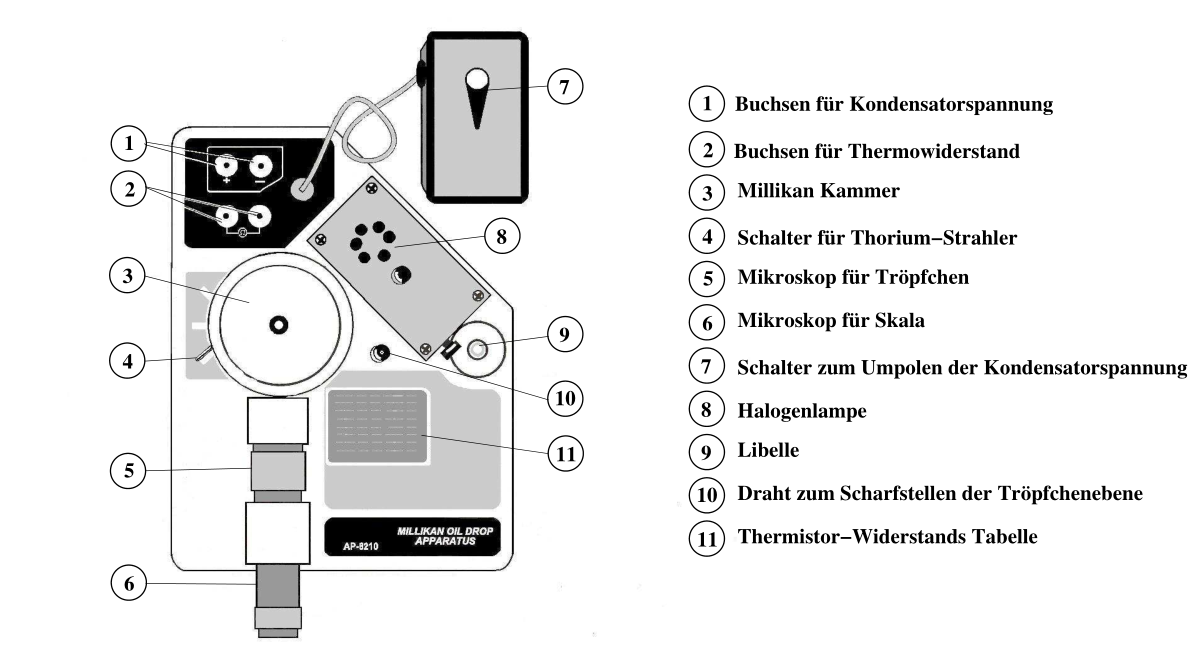
\includegraphics[height=8cm]{ressources/aufbau.png}
  \caption{Schematische Ansicht des Versuchsaufbaus von oben. \cite{skript}}
  \label{millikan}
\end{figure}


Den Kern des Aufbaus bildet die Millikan-Kammer.
Es handelt sich hierbei um einen Plattenkondensator senkrecht zur Erdanziehungskraft, was über eine integrierte Libelle erkennbar ist.
Er ist oben mit einer Öffnung versehen, welche einen Zugang zwischen die beiden Kondensatorplatten ermöglicht.
Diese werden von einer regelbaren Spannung gespeist, wobei die Orientierung des Feldes über einen Kippschalter geändert werden kann.
Über einen Thermowiederstand kann die Temperatur innerhalb der Millikan-Kammer abgelesen werden.
Die Kammer wird mit Öltröpfchen über einen Zerstäuber durch den Zugang der Kammer befüllt.
Diese können über Ioniserung der umgebenen Luft durch ein Alpha-Präparat, welches über einen weiteren Kippschalter an die Kammer gekoppelt werden kann, negativ geladen werden.
Zur Beobachtung der Öltröpfchen sind zusätzlich eine Lichtquelle und ein Kamera-Linsensystem an der Kammer angebracht.
Das Linsensystem ist einstellbar und am Ende mit einer Skala versehen.
Das aufgenommene Bild ist auf einem Schirm beobachtbar.
